\documentclass{article}

\usepackage[T1]{fontenc}
\usepackage[utf8]{inputenc}
\usepackage{graphicx}
\usepackage{caption}
\usepackage[font=small,labelfont=bf]{caption}
\usepackage{booktabs, siunitx}
\usepackage{tikz}
\usepackage{tikz-qtree}
\usepackage{pifont}
\usepackage[margin=0.90in]{geometry}
\usepackage{etoolbox,titling}
\usepackage{enumitem}
\usepackage{fancyhdr}
\usepackage{soulutf8}
\usepackage{epigraph}
\usepackage{amssymb}
\usepackage{amsmath}

\pagestyle{fancy}
\fancyhf{}
\rhead{Virginia Filippi e Chiara Solito}
\lhead{VaccineSupervision}
\rfoot{Pagina \thepage}
\lfoot{Bioinformatica - A.A. 2021/22}
\usetikzlibrary{trees}
\tikzstyle{every node}=[draw=black,thick,anchor=west]
\newcommand{\angstrom}{\mbox{\normalfont\AA}}

\begin{document}
\newcommand\tab[1][0.3cm]{\hspace*{#1}}


\begin{titlepage}
    \begin{center}
        \vspace*{1cm}
            
        \Huge
        \textbf{Vaccine Supervision}
            
        \vspace{0.5cm}
        \LARGE
        Progetto di Ingegneria del Software
            
        \vspace{1.5cm}
            
        \textbf{Virginia Filippi e Chiara Solito}

        \vspace{0.8cm}

            
        \Large
        Corso di Laurea in Bioinformatica\\
        Università degli studi di Verona\\
        A.A. 2021/22
            
    \end{center}
\end{titlepage}
La presente è la documentazione blablabla.\\
Insieme a questo documento in formato PDF viene fornito anche il codice \LaTeX  con cui è stato generato.
\tableofcontents
\thispagestyle{empty}
\newpage
\thispagestyle{empty}

\section{Traccia dell'Elaborato}
Riportiamo di seguito la traccia dell'elaborato:
\begin{quotation}
    Si vuole progettare un sistema software per gestire le segnalazioni di reazioni avverse (ad esempio, asma, dermatiti, insufficienza renale, miocardiopatia, \dots) da vaccini anti-Covid.\\
    Ogni segnalazione è caratterizzata da un codice univoco, dall'indicazione del paziente a cui fa riferimento, dall'indicazione della reazione avversa, dalla data della reazione avversa, dalla data di segnalazione, e dalle vaccinazioni ricevute nei due mesi precedenti il momento della reazione avversa.
    Per ogni paziente sono memorizzati: un codice univoco, l'anno di nascita, la provincia di residenza e la professione.\\
    Per ogni paziente è possibile memorizzare gli eventuali fattori di rischio presenti (paziente fumatore, iperteso, sovrappeso, paziente fragile per precedenti patologie cardiovascolari/oncologiche), anche più d'uno. Ogni fattore di rischio è caratterizzato da un nome univoco, una descrizione e il livello di rischio associato. Per ogni paziente è, inoltre, memorizzata l'intera storia delle sue vaccinazioni precedenti, anti-Covid-19 e antinfluenzali.\\
    Ogni vaccinazione è caratterizzata da: paziente a cui si riferisce, segnalazioni a cui è legata, vaccino somministrato (AstraZeneca, Pfizer, Moderna, Sputnik, Sinovac, antinfluenzale, \dots), tipo della somministrazione (I, II, III o IV dose, dose unica), sede presso la quale è avvenuta la vaccinazione e data di vaccinazione. Per ogni reazione avversa sono memorizzati un nome univoco, un livello di gravità (da 1 a 5) e una descrizione generale, espressa in linguaggio naturale. Una reazione avversa può essere legata a molte segnalazioni. Per ogni paziente sono memorizzati il numero di reazioni avverse segnalate ed il numero di vaccinazioni ricevute.\\
    Il sistema deve supportare i medici che effettuano la segnalazione. Dopo opportuna autenticazione, il medico viene introdotto ad una interfaccia che permette l'inserimento dei dati delle reazioni avverse e dei pazienti. Il codice univoco dei pazienti è gestito dal sistema, che tiene traccia dei pazienti indicati da ogni medico. Ogni medico vede solo i codici identificativi dei pazienti, dei quali ha già segnalato qualche reazione avversa, e le relative informazioni.\\
    Ad ogni fine settimana o quando il numero di segnalazioni raggiunge la soglia di 50, il sistema manda un avviso ad uno dei farmacologi responsabili della gestione delle segnalazioni di reazioni avverse. Il farmacologo, dopo autenticazione, accede alle segnalazioni (tutte, con l'indicazione del medico che le ha fatte) e può effettuare alcune analisi di base (quante segnalazioni per vaccino, quante segnalazioni gravi in settimana, quante segnalazioni per provincia e quante segnalazioni per sede di vaccinazione). Il sistema, inoltre, avvisa il farmacologo quando un vaccino ha accumulato in un mese oltre 5 segnalazioni di gravità superiore a 3.
    In base alle segnalazioni e agli avvisi del sistema, il farmacologo può proporre di attivare una fase di controllo del vaccino. Tale proposta viene registrata dal sistema, che tiene traccia di tutte le proposte relative ai vaccini segnalati.
\end{quotation}

\section{Analisi e Specifica dei Requisiti}
\subsection{Specifiche casi d'uso}
In questa sezione definiamo le proprietà dell'applicazione.\\
Come dichiarato nella traccia il sistema prevede l'utilizzo da parte di due tipologie di personale medico: Medico e Farmacologo. 
Entrambi i tipi di utente possono utilizzare l'applicazione dopo opportuno login: in questa sede si è previsto che gli utenti siano pre-registrati da un amministratore di sistema esterno (sul modello di sistemi medici già noti). Non è stato quindi previsto un form di registrazione, durante lo sviluppo e si suppone che ogni utente abbia a disposizione \texttt{username} e \texttt{password}.

\newpage
\paragraph*{Casi d'uso relativi al Medico}
\begin{center}
    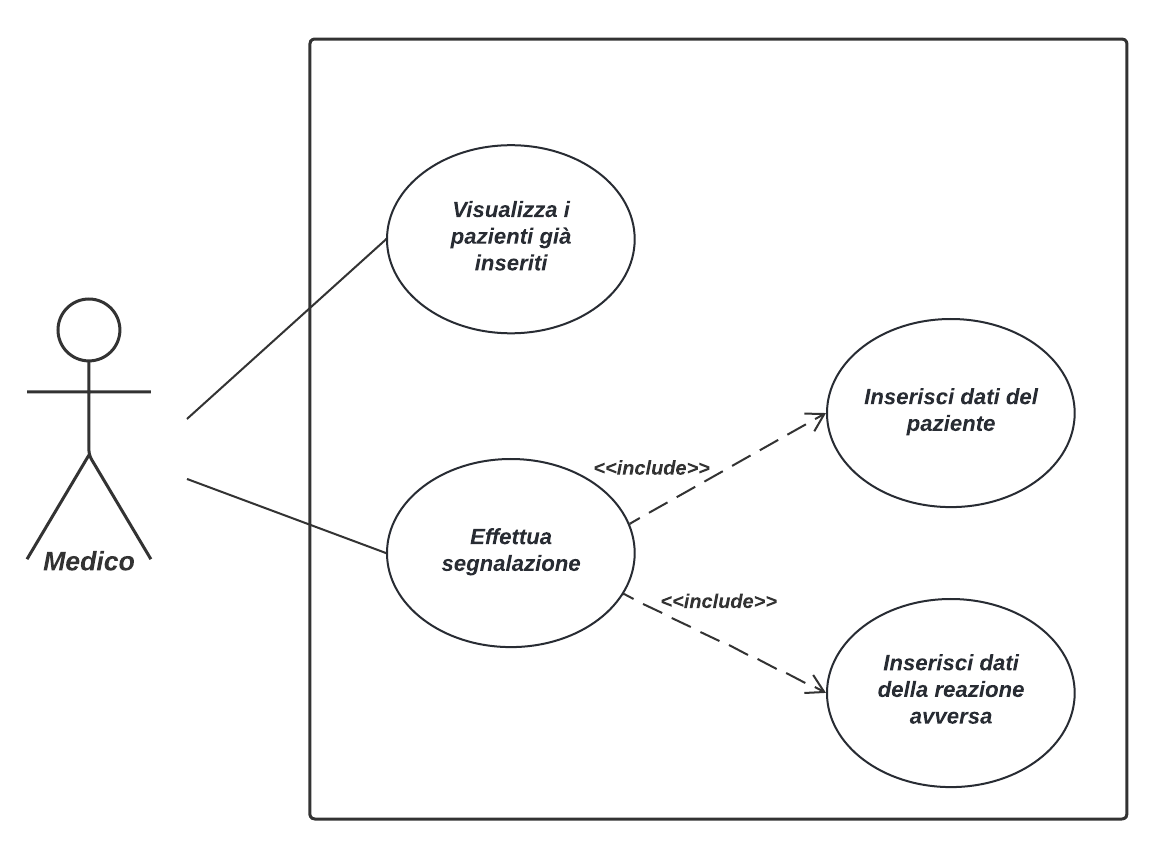
\includegraphics[width=0.75\textwidth]{pictures/CasoDUsoMedico.png}
\captionof{figure}{Caso d'uso Medico}
\end{center}
Dopo opportuna autenticazione il medico viene introdotto all'interfaccia di base della sua sezione, che gli permette di:
\begin{itemize}
    \item Visualizzare i pazienti già inseriti.
    \item Visualizzare i dati di un paziente, dalla lista dei pazienti già inseriti.
    \item Effettuare una segnalazione.
\end{itemize}
\subparagraph*{Visualizza i pazienti}
Una delle possibili attività che il Medico è autorizzato a fare è visualizzare la lista dei codici dei pazienti che lui stesso ha già inserito (gestiti automaticamente dal sistema), effettuando una segnalazione.
\begin{center}
    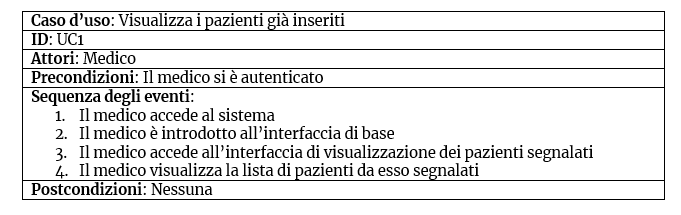
\includegraphics[width=0.75\textwidth]{pictures/UC1.png}
\captionof{figure}{Caso d'uso UC1 del Medico}
\end{center}

\newpage
Il medico può visualizzare anche le informazioni relative ai pazienti di cui vede i codici:
\begin{center}
    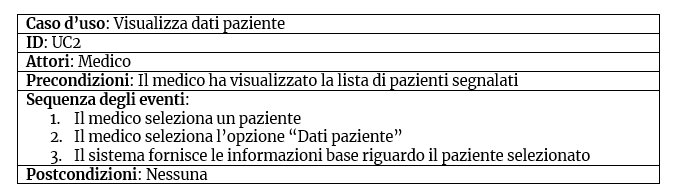
\includegraphics[width=0.75\textwidth]{pictures/UC2.png}
\captionof{figure}{Caso d'uso UC2 del Medico}
\end{center}
Inseriamo ulteriori dettagli rispetto a questi due casi d'uso (gestiti in unico Sequence Diagram).
\begin{center}
    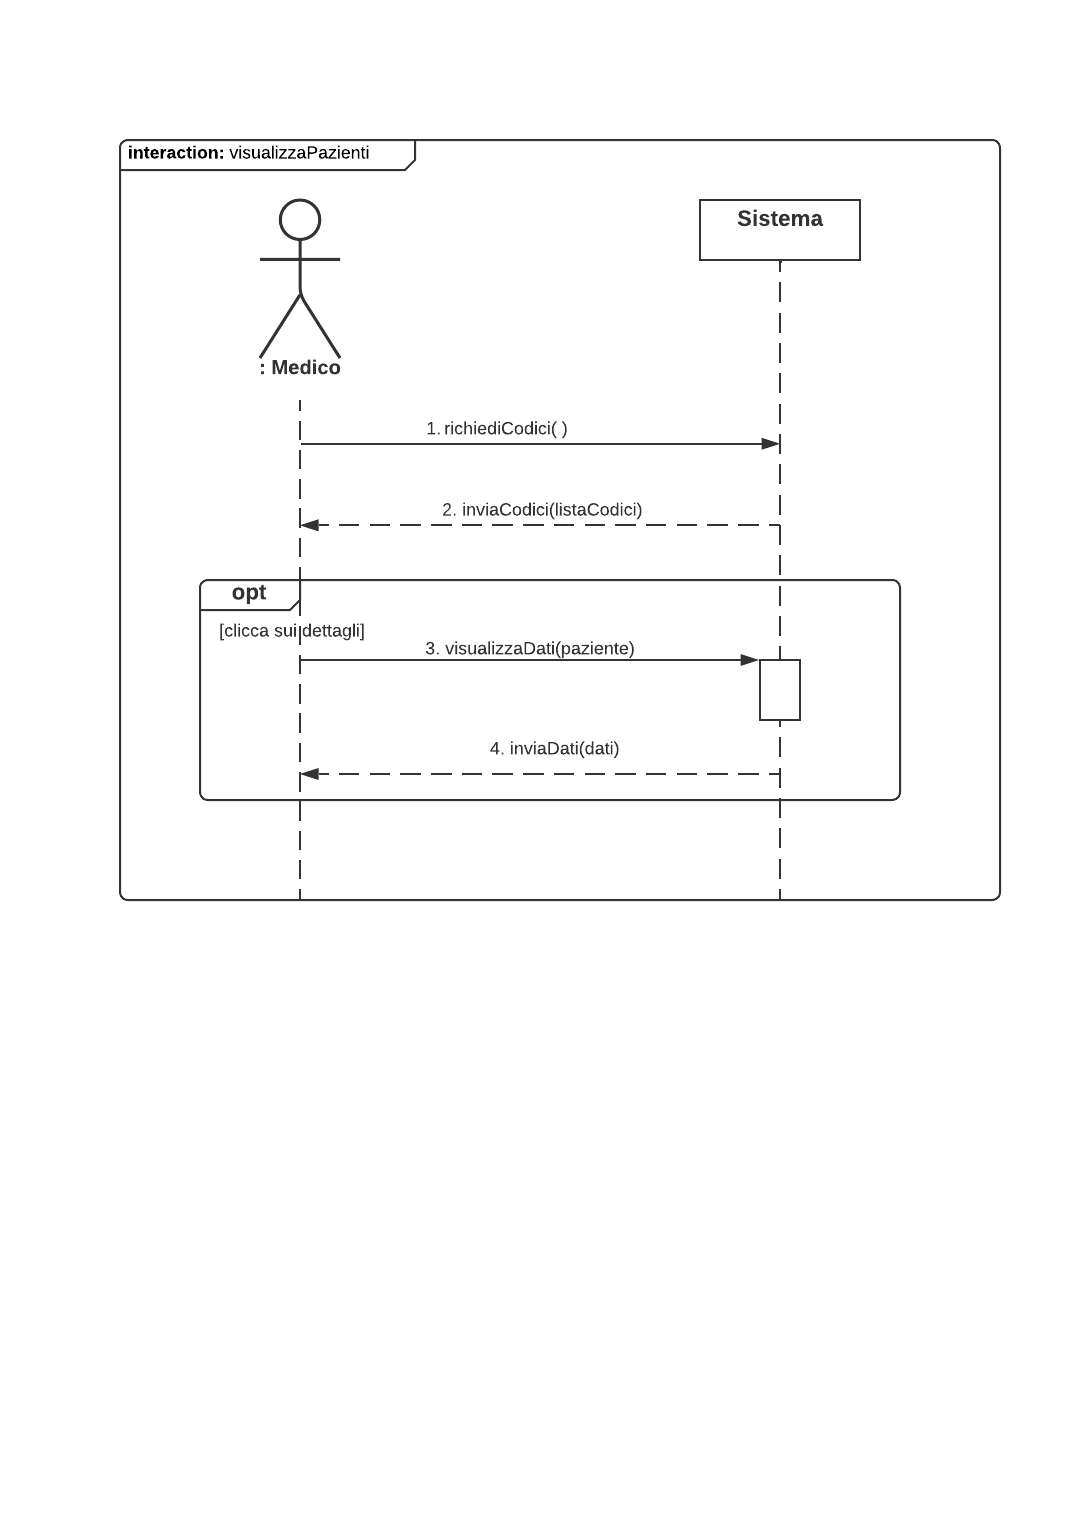
\includegraphics[width=0.80\textwidth]{pictures/SDMedico2_listaPazienti.png}
\captionof{figure}{Sequence Diagram Visualizza Pazienti}
\end{center}

\newpage
\subparagraph*{Effettua segnalazione}
La principale attività dei medici è quella di inserire segnalazioni. Per fare questo, è necessario
inserire i \textbf{dati del paziente} ed inserire i \textbf{dati della reazione avversa}. In questa sede si è scelto di dare uno specifico ordine a queste due azioni.\\
La data della segnalazione può essere gestita automaticamente oppure modificata dal medico.
\begin{center}
    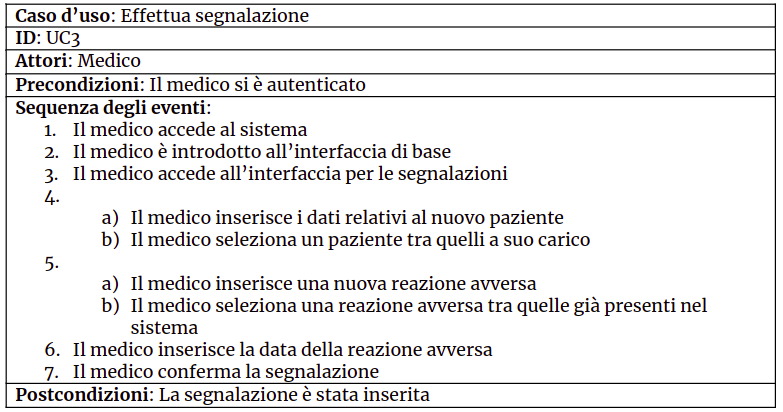
\includegraphics[width=0.65\textwidth]{pictures/UC3.png}
\captionof{figure}{Caso d'uso UC3 del Medico}
\end{center}
In questa fase prevediamo che il primo passo sia inserire i dati del paziente, abbiamo due alternative:
\begin{itemize}
    \item Inserire nuovi dati del paziente, effettuando quindi l'intera procedura di inserimento (dati anagrafici, fattori di rischio e storia vaccinale)
    \item Scegliere uno dei pazienti già inseriti nel sistema.
\end{itemize}
L'identificativo univoco del paziente sarà gestito dal sistema.\\
Subito dopo si inseriscono i dati sulla reazione avversa.
Anche in questa fase prevediamo le due alternative:
\begin{itemize}
    \item Inserimento in sistema di una nuova reazione avversa, immettendo nome (univoco), gravità e descrizione.
    \item Selezione di una reazione avversa nota, pre-esistente nel sistema, aggiungendo la data.
\end{itemize}
Si prevede quindi che, data la storia vaccinale del paziente e la data della segnalazione, il sistema gestisce autonomamente
le vaccinazioni del paziente entro i due mesi precedenti la segnalazione.

\newpage
In ambo i casi, sarà necessario inserire la data della reazione avversa: questa dovrà essere consistente sia con la data della segnalazione sia con la data delle terapie del paziente.
\begin{center}
    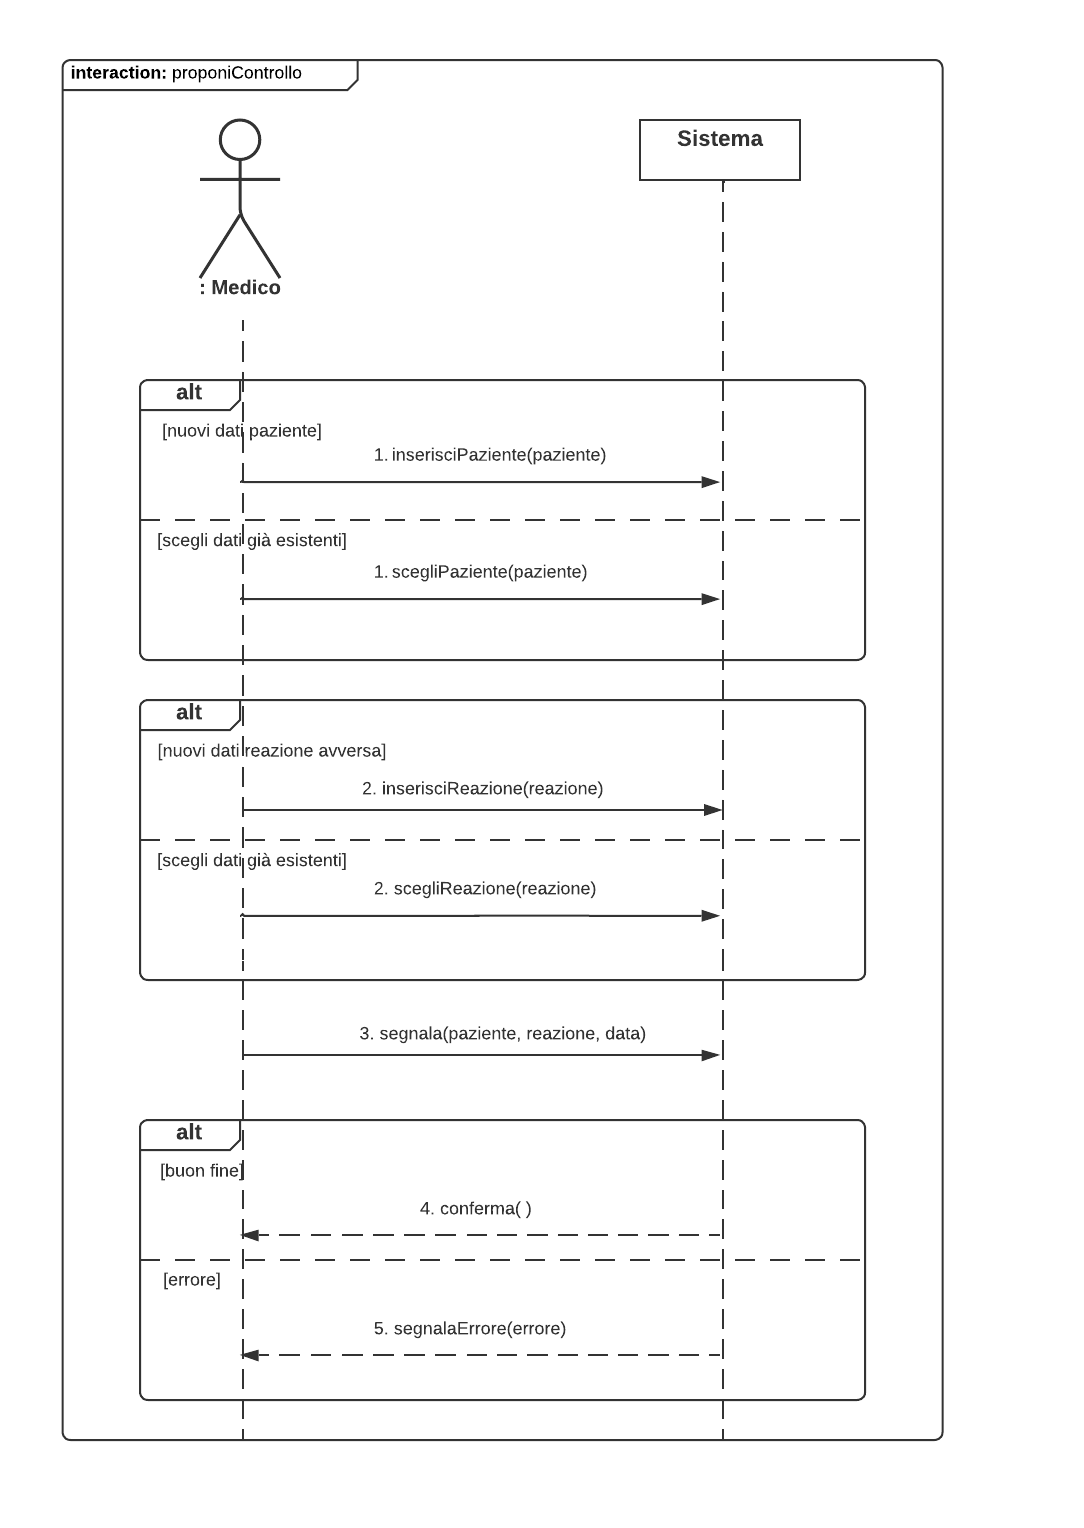
\includegraphics[width=0.80\textwidth]{pictures/SDMedico1_Segnalazione.png}
\captionof{figure}{Sequence Diagram Effettua Segnalazione}
\end{center}

\newpage
\paragraph*{Casi d'uso relativi al Farmacologo}
\begin{center}
    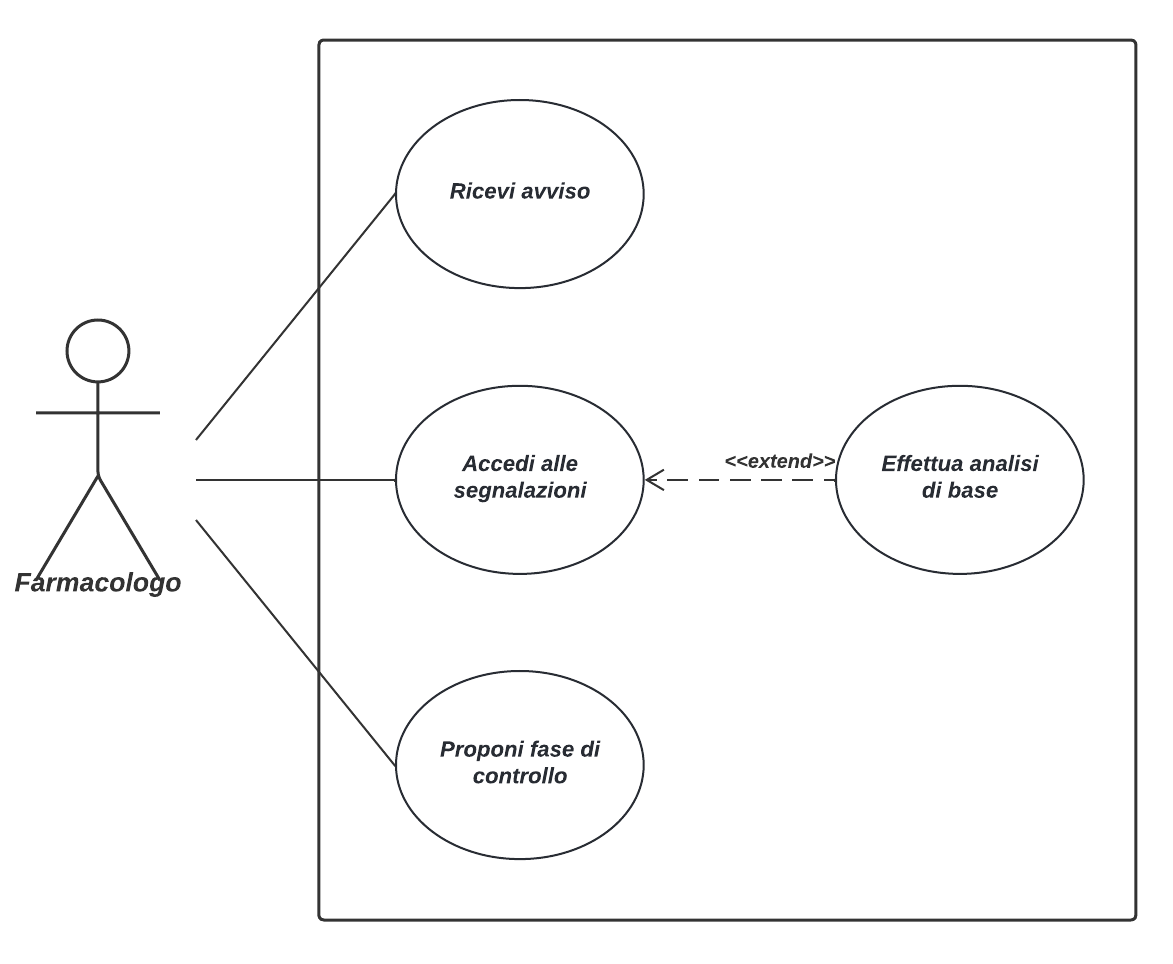
\includegraphics[width=0.75\textwidth]{pictures/CasoDUsoFarmacologo.png}
\captionof{figure}{Caso d'uso Farmacologo}
\end{center}
Dopo opportuna autenticazione il farmacologo viene introdotto all'interfaccia di base della sua sezione. Prima di poter effettuare qualsiasi azione gli vengono mostrati gli \textbf{avvisi non letti}. Dopo di che egli può:
\begin{itemize}
    \item Accedere alle segnalazioni
    \item Dalle segnalazioni può effettuare delle analisi di base
    \item Proporre delle fasi di controllo
\end{itemize}
\subparagraph*{Avvisi}
Iniziamo dalla ricezione degli avvisi.\\
Il sistema deve fornire un meccanismo di gestione ed invio di avvisi verso i
farmacologi, che si dividono in tre tipologie:
\begin{enumerate}
    \item Il sistema manda un avviso non specifico se sono state raggiunte le 50 segnalazioni in una settimana.
    \item Il sistema manda un avviso non specifico se è il weekend.
    \item Il sistema manda un avviso specifico rispetto a un vaccino, se questo ha accumulato oltre 5 segnalazioni di gravità superiore a 3.
\end{enumerate}
Il sistema avverte \textbf{tutti} i farmacologi responsabili. Ciò significa che ogni farmacologo all'autenticarsi riceverà gli avvisi generati e non ancora letti \textit{da lui}:
questo avviene in forma di pop-up e prima di vedere la schermata iniziale. È inoltre possibile, tramite un'opzione nel menù principale, rivedere gli avvisi già letti.
\begin{center}
    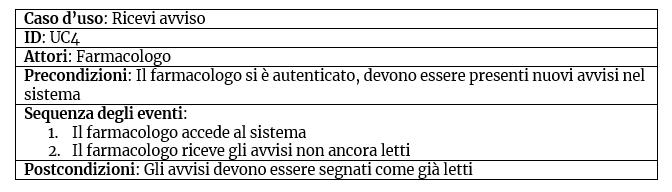
\includegraphics[width=0.75\textwidth]{pictures/UC4.png}
\captionof{figure}{Caso d'uso UC4 del Farmacologo}
\end{center}
In fase di descrizione dei casi d'uso si è ritenuto opportuno inserire anche la possibilità di vedere gli avvisi già letti, sulla base dei quali il farmacologo propone le fasi di controllo:
\begin{center}
    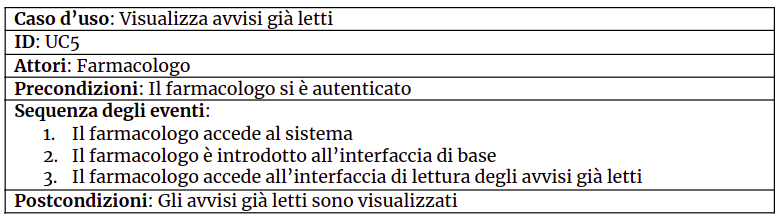
\includegraphics[width=0.75\textwidth]{pictures/UC5.png}
\captionof{figure}{Caso d'uso UC5 del Farmacologo}
\end{center}
\subparagraph*{Leggi Segnalazioni}
Il farmacologo può accedere alla lista delle segnalazioni:
\begin{center}
    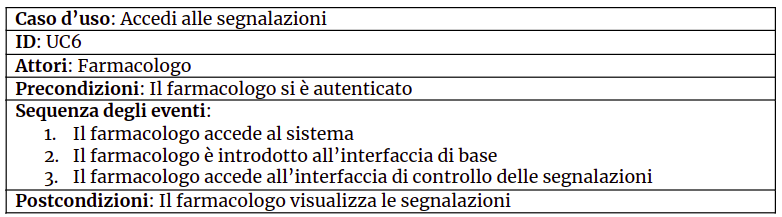
\includegraphics[width=0.75\textwidth]{pictures/UC6.png}
\captionof{figure}{Caso d'uso UC6 del Farmacologo}
\end{center}
Si è previsto che, come il medico visualizza informazioni di base dalla lista dei pazienti, anche il farmacologo possa visualizzare informazioni di base sulle segnalazioni. 

\newpage
Questo è stato specificato nel sequence diagram qui inserito:
\begin{center}
    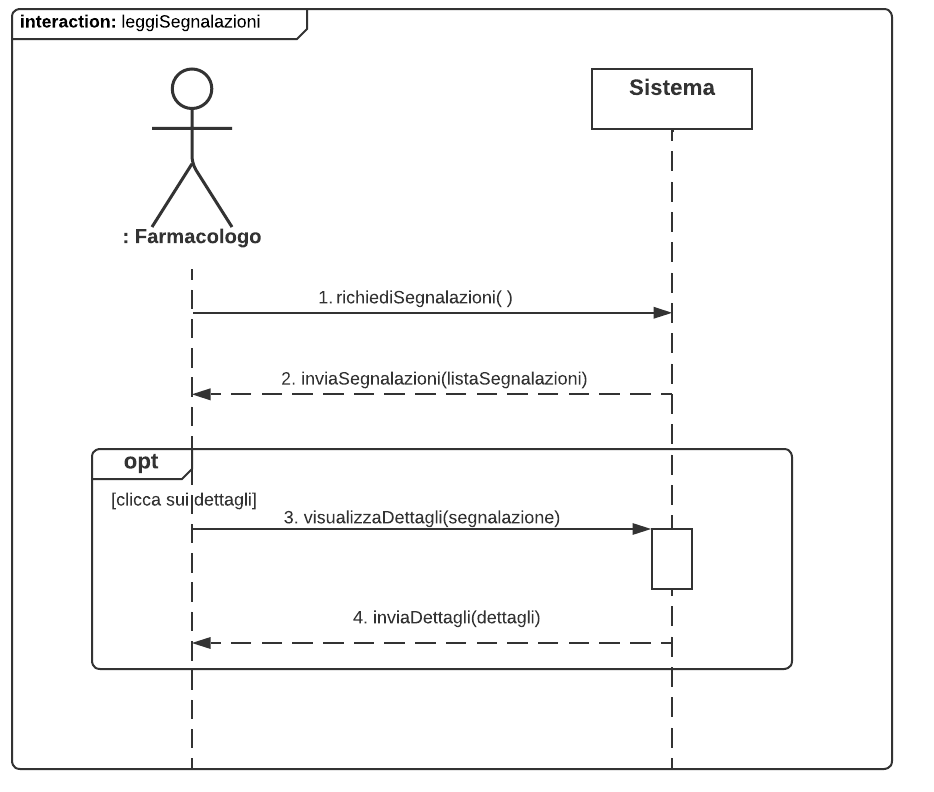
\includegraphics[width=0.75\textwidth]{pictures/SDFarmacologo1_Segnalazioni.png}
\captionof{figure}{Sequence Diagram 1 Farmacologo}
\end{center}
\subparagraph*{Effettua analisi di base}
Dalla lista delle segnalazioni può scegliere di effettuare delle \textbf{analisi di base}. Queste sono:
\begin{itemize}
    \item Quante segnalazioni per vaccino
    \item Quante segnalazioni gravi in settimana
    \item Quante segnalazioni per provincia 
    \item Quante segnalazioni per sede di vaccinazione
\end{itemize}
\begin{center}
    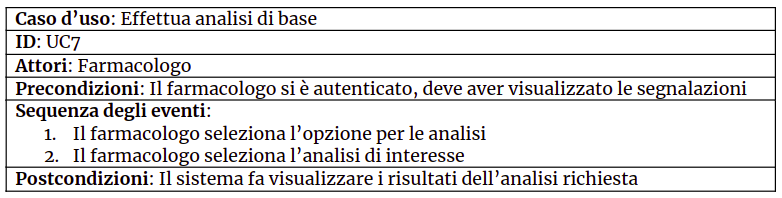
\includegraphics[width=0.75\textwidth]{pictures/UC7.png}
\captionof{figure}{Caso d'uso UC7 del Farmacologo}
\end{center}

\newpage
\subparagraph*{Propone Fase di Controllo}
In base alle analisi eseguite e alla lettura delle segnalazioni, il farmacologo può proporre di attivare una fase di controllo del vaccino.\\
Tale proposta viene registrata dal sistema.
\begin{center}
    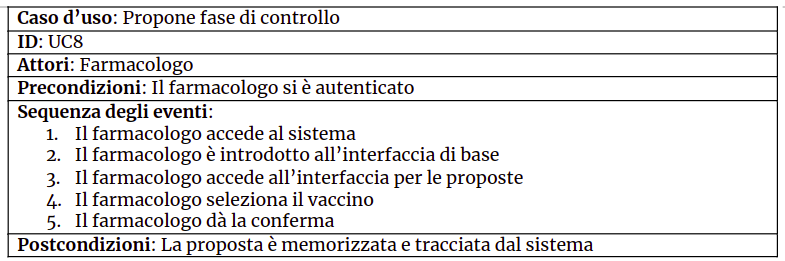
\includegraphics[width=0.75\textwidth]{pictures/UC8.png}
\captionof{figure}{Caso d'uso UC8 del Farmacologo}
\end{center}
Di seguito un Sequence Diagram specifica queste azioni:
\begin{center}
    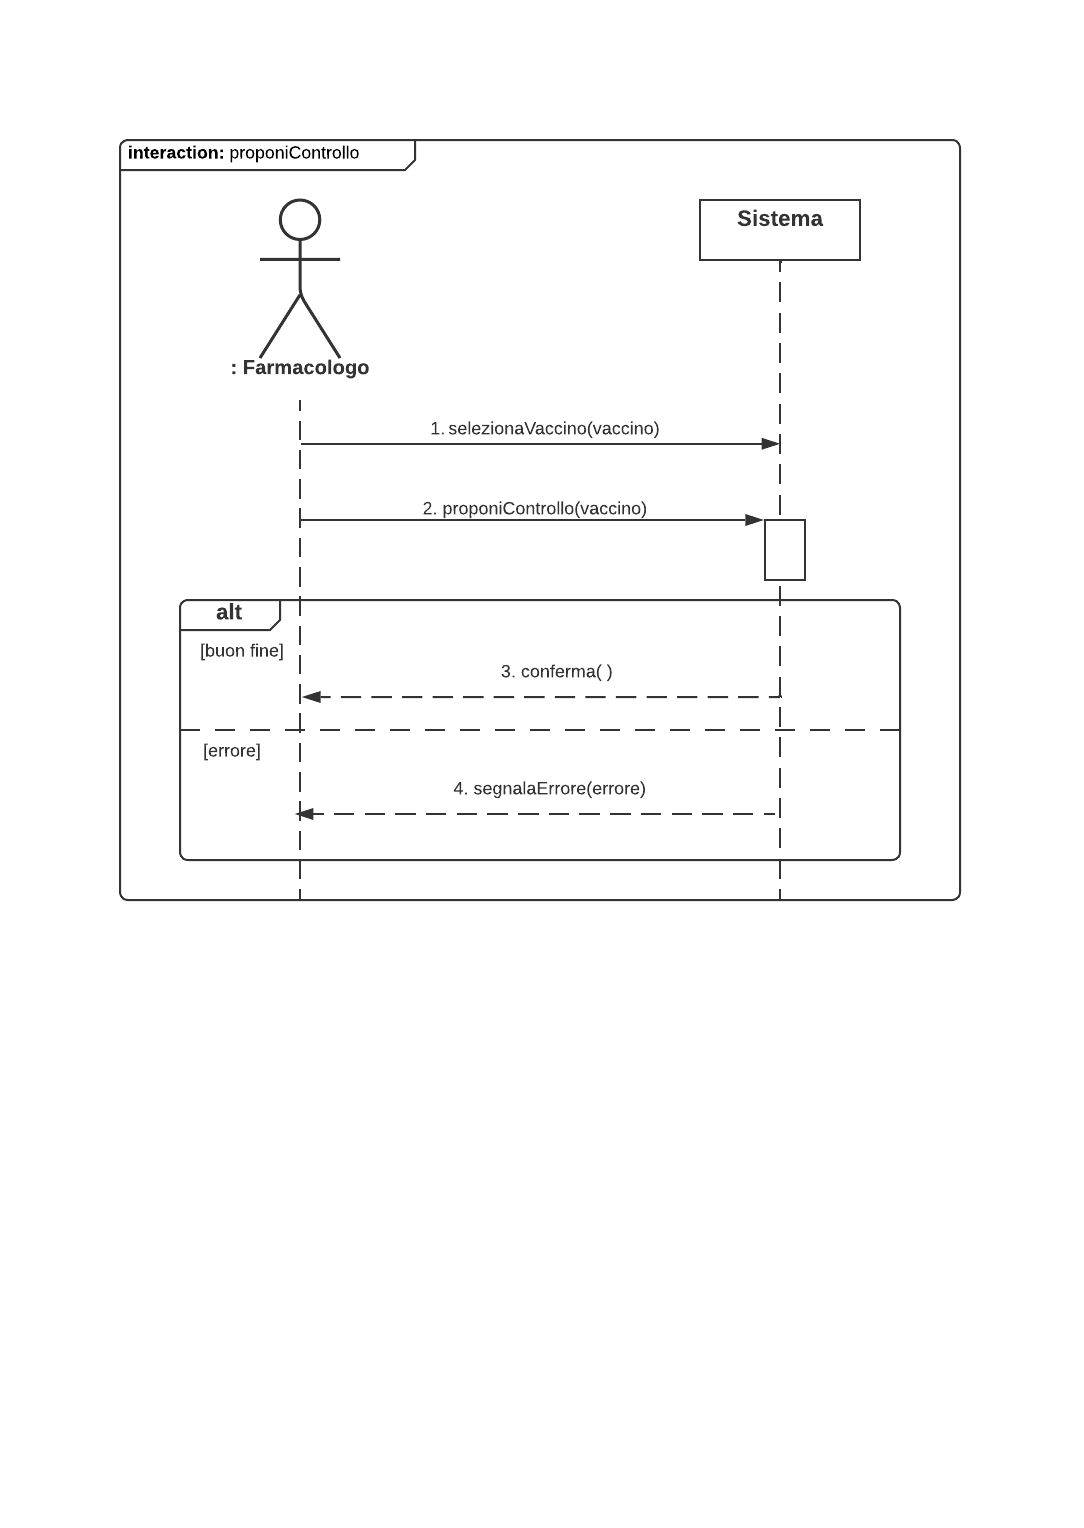
\includegraphics[width=0.80\textwidth]{pictures/SDFarmacolo2_proponeControllo.png}
\captionof{figure}{Sequence Diagram 2 Farmacologo}
\end{center}

\newpage
\subsection{Diagrammi di Attività}
\paragraph*{Nota sui diagrammi}
Nei diagrammi relativi alle azioni successive al login non si è ritenuto di aggiungere una freccia che collega la scelta finale ad ogni interfaccia di partenza, per chiarezza e compattezza degli schemi.\\

\paragraph*{Attività di Login}
\begin{center}
    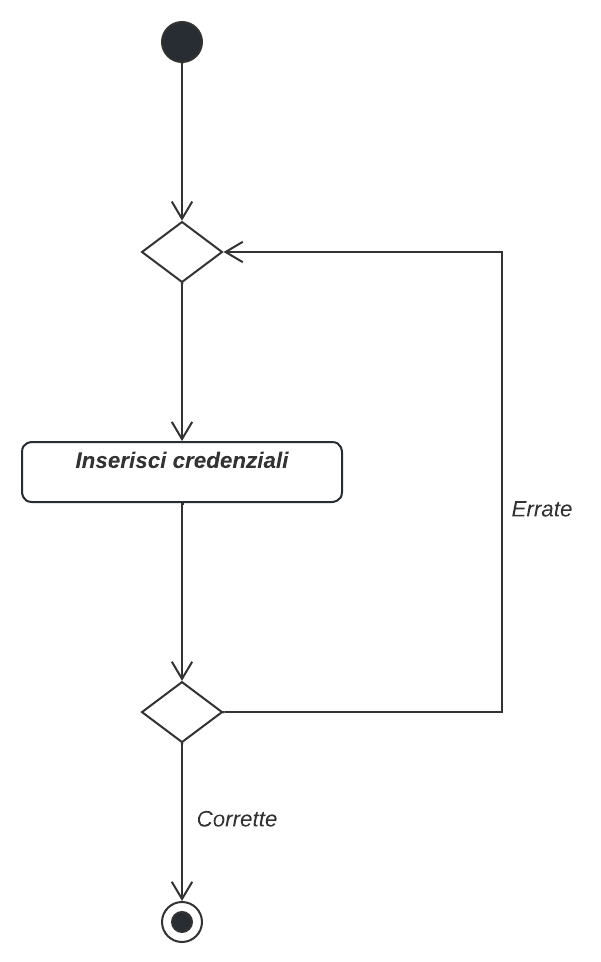
\includegraphics[width=0.60\textwidth]{pictures/ActivityDiagram_Login.png}
\captionof{figure}{}
\end{center}

\newpage
\paragraph*{Attività dell'attore medico}
\begin{center}
    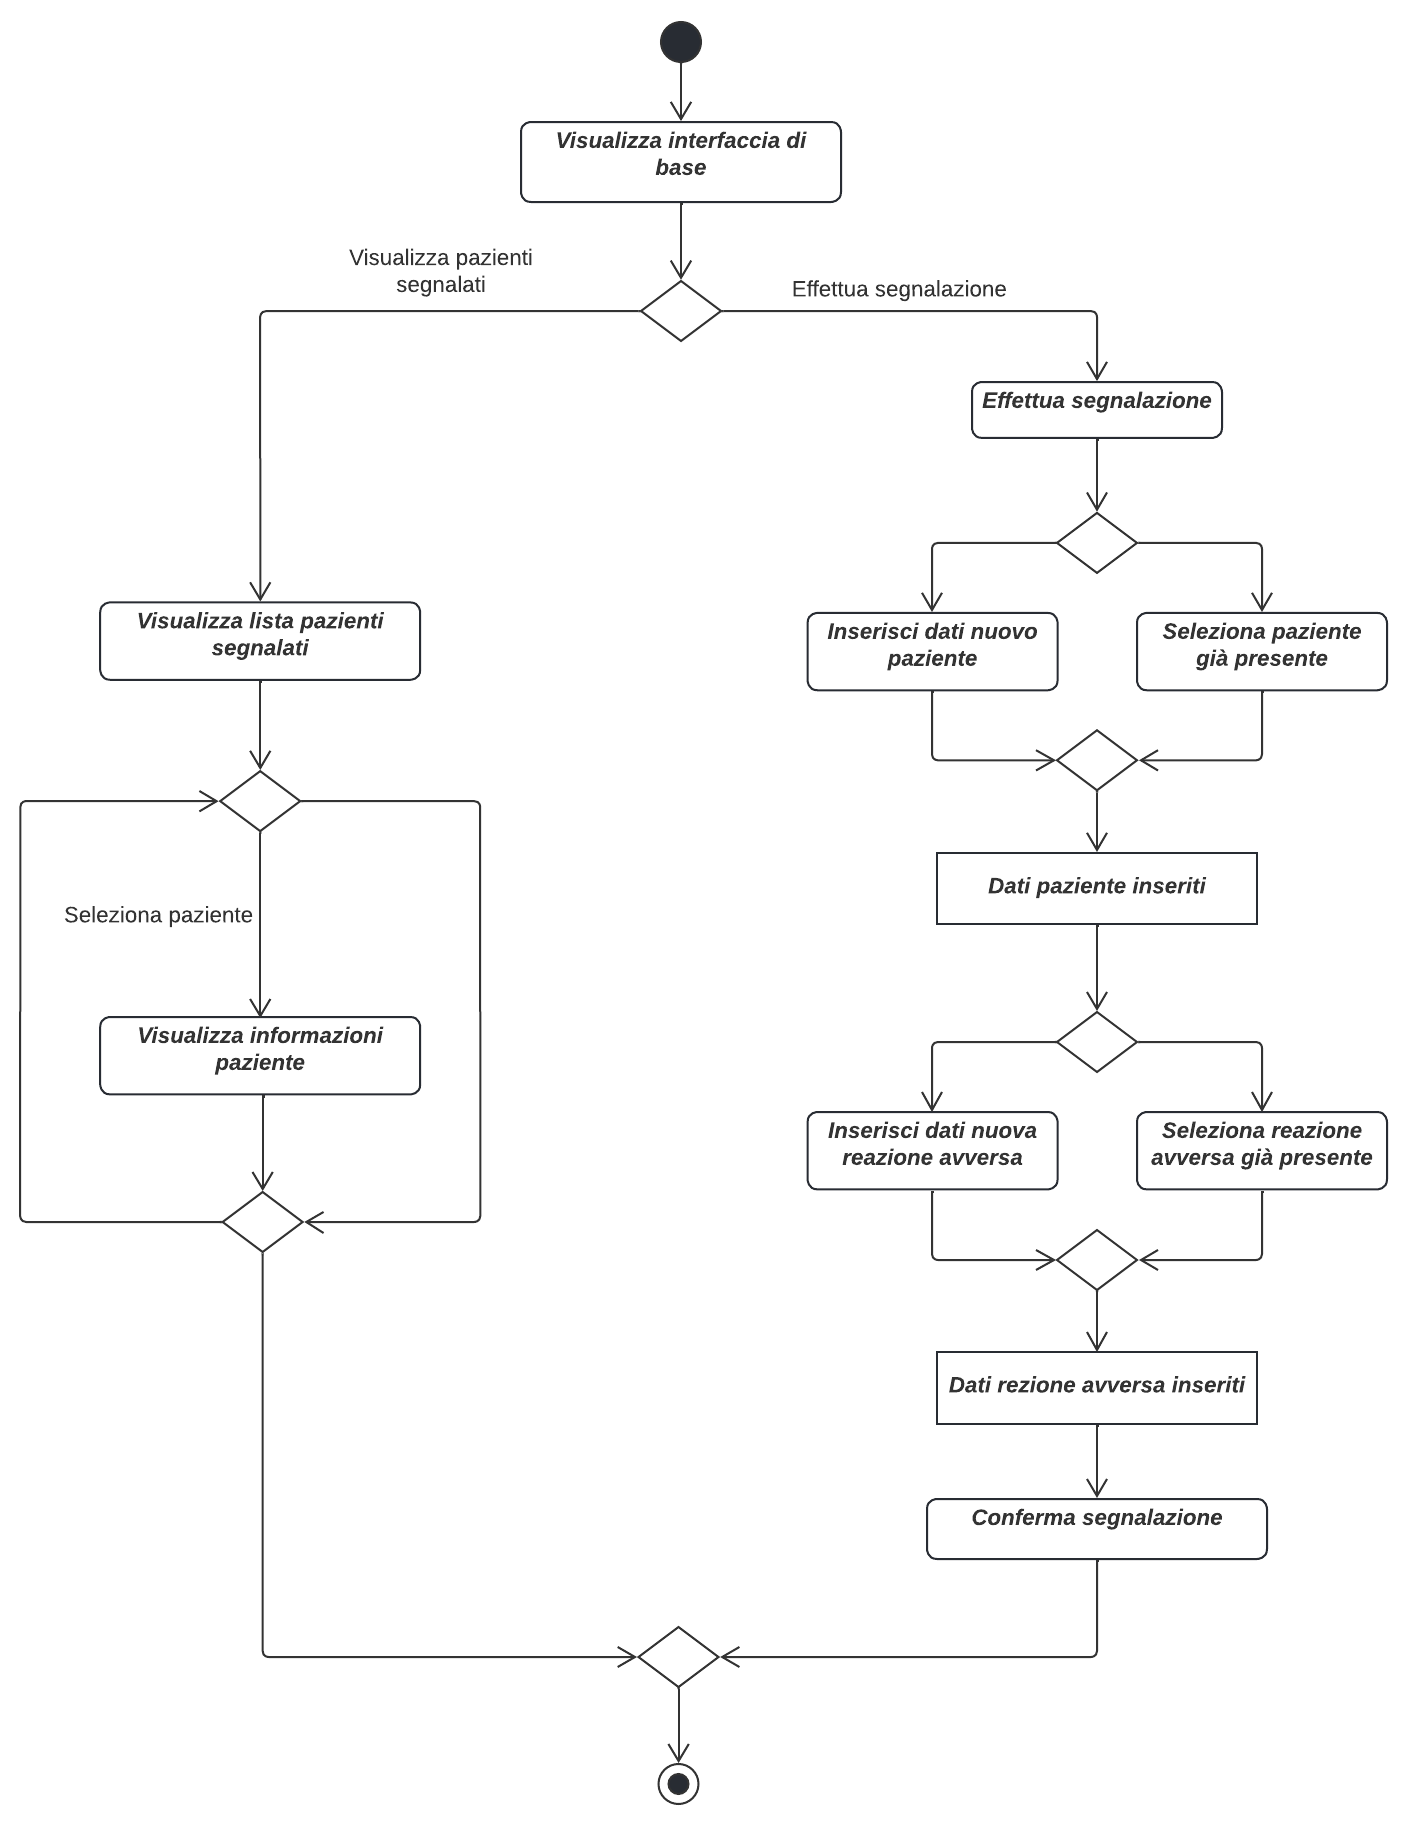
\includegraphics[width=1\textwidth]{pictures/ActivityDiagram_Medico.png}
\captionof{figure}{}
\end{center}

\newpage
\paragraph*{Attività dell'attore farmacologo}
\begin{center}
    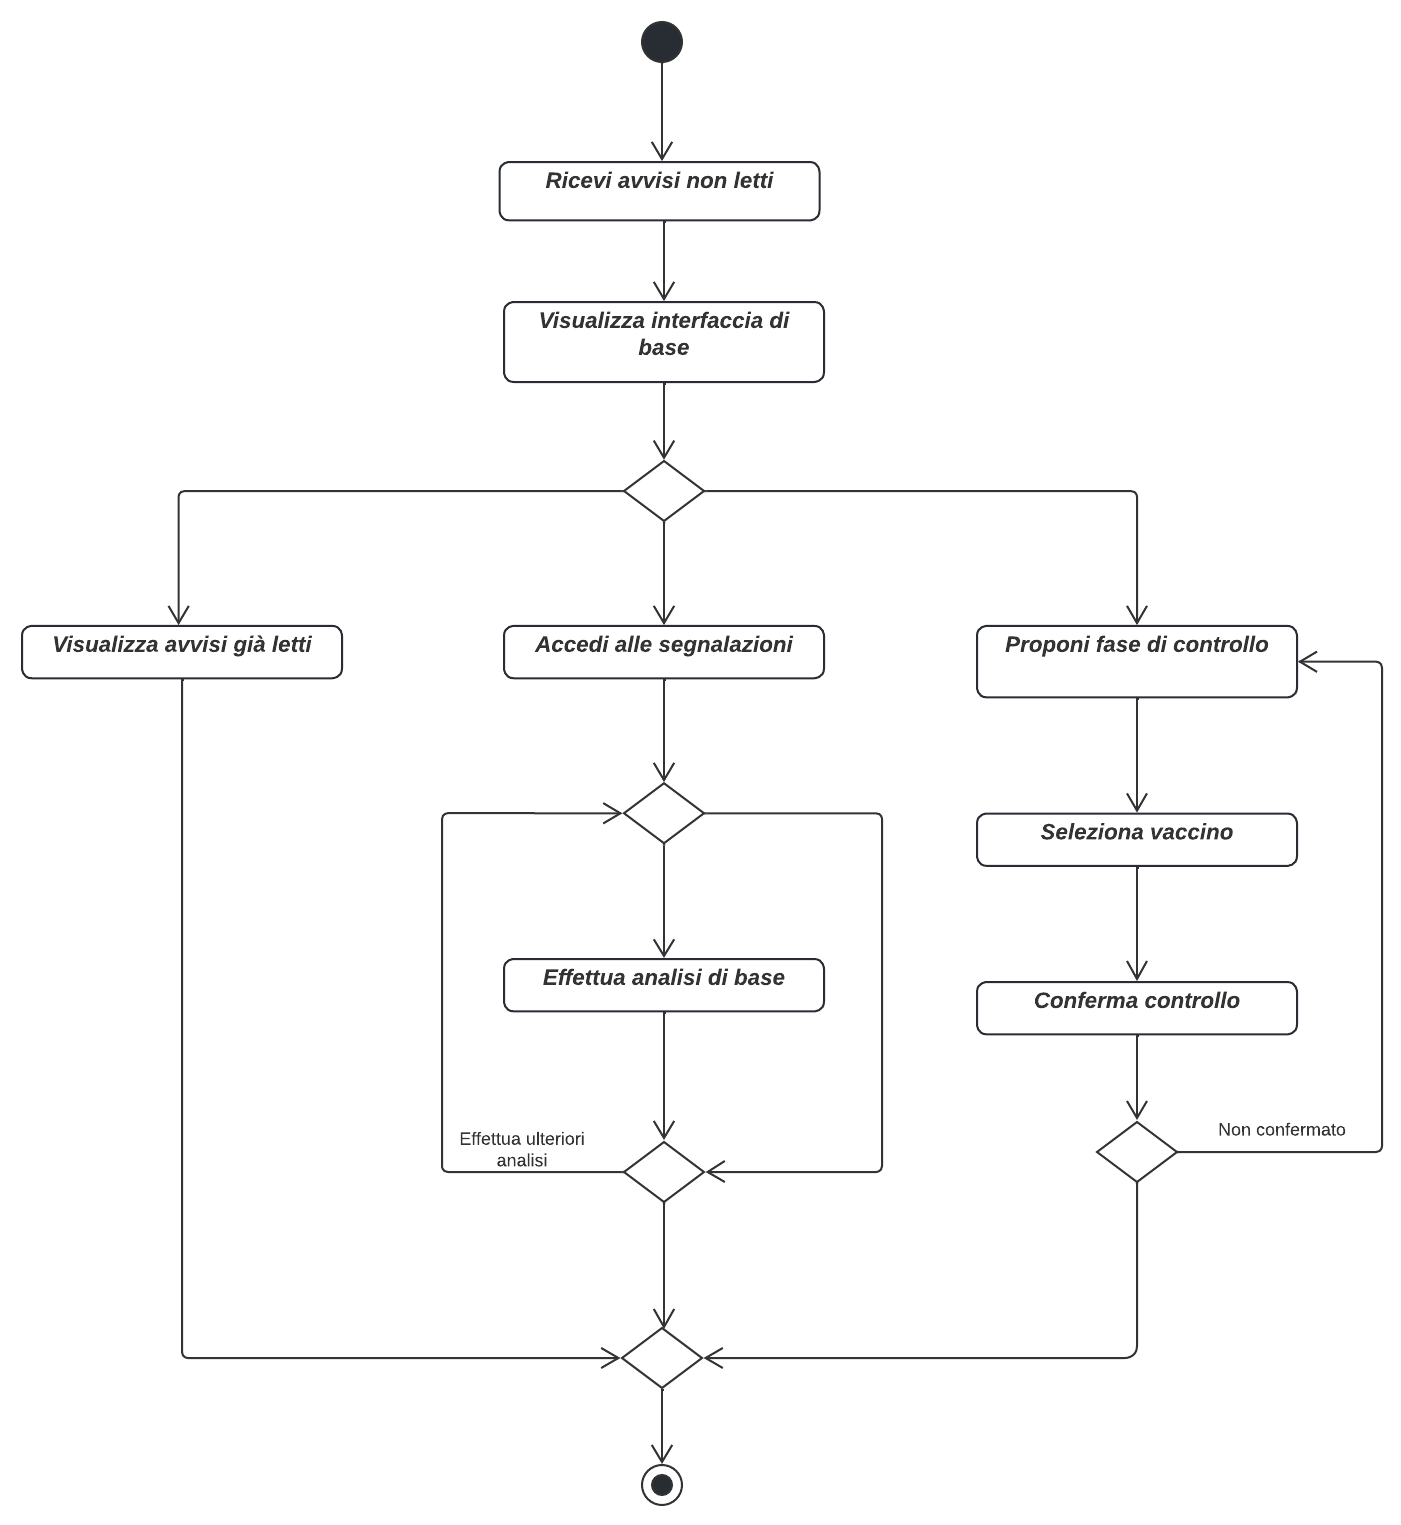
\includegraphics[width=1\textwidth]{pictures/ActivityDiagram_Farmacologo.png}
\captionof{figure}{}
\end{center}

\newpage
\section{Scelte progettuali}
\subsection{Note sullo sviluppo}
Si è scelto di sviluppare l'applicazione in Java, utilizzando la libreria \textbf{JavaFX}, senza l'ausilio di FXML, perché soddisfatti del design delle interfacce.\\
Il progetto è stato interamente sviluppato utilizzando \textbf{Git} come sistema di \textit{code versioning} e GitHub per l'hosting della repository.\\
Abbiamo seguito una metodologia di sviluppo per lo più a cascata e \textbf{Plan Driven}: le fasi di specifica e di sviluppo sono state separate, cercando di porre comunque rimedio al principale svantaggio dello stesso, ovvero la difficoltà di cambiamento dopo aver avviato il processo. Questo è stato fatto utilizzando alcune metodologie proprie dello \textbf{sviluppo Agile}, soprattutto l'attività di \textit{Pair Programming} che ha riguardato tutto lo sviluppo, con particolare attenzione allo sviluppo dei Modelli e delle prime View (si veda in seguito).\\
Ogni area è stata divisa in task in modo da alleggerire il carico di lavoro e i design pattern sono stati scelti nella fase di sviluppo in base a quelle che erano le nostre necessità, al fine di ottenere un codice performante ma allo stesso tempo leggibile.\\
Prima di cominciare lo sviluppo vero e proprio, si è condotta la fase di analisi dei requisiti che si è vista nella sezione precedente, generando i relativi use-cases e i diagrammi di attività. Anche la progettazione architetturale è stata fatta prima di iniziare il lavoro centrale, in
modo da non avere problemi su quel frangente.
\subsection{Pattern Architetturale - MVC}
Abbiamo deciso di utilizzare il \textbf{pattern Model View Controller}, semplicemente perchè naturalmente implementabile con l'uso di JavaFX. Il sistema è strutturato in tre componenti logiche che interagiscono tra loro. Il \textbf{model} si occupa della gestione dei dati e delle operazioni su di essi. La componente \textbf{View} definisce le interfazze e come i dati vengono presentati all'utente. Il \textbf{Controller} 
gestisce infine l'interazione delle interfacce e dell'utente con i dati.
\begin{center}
    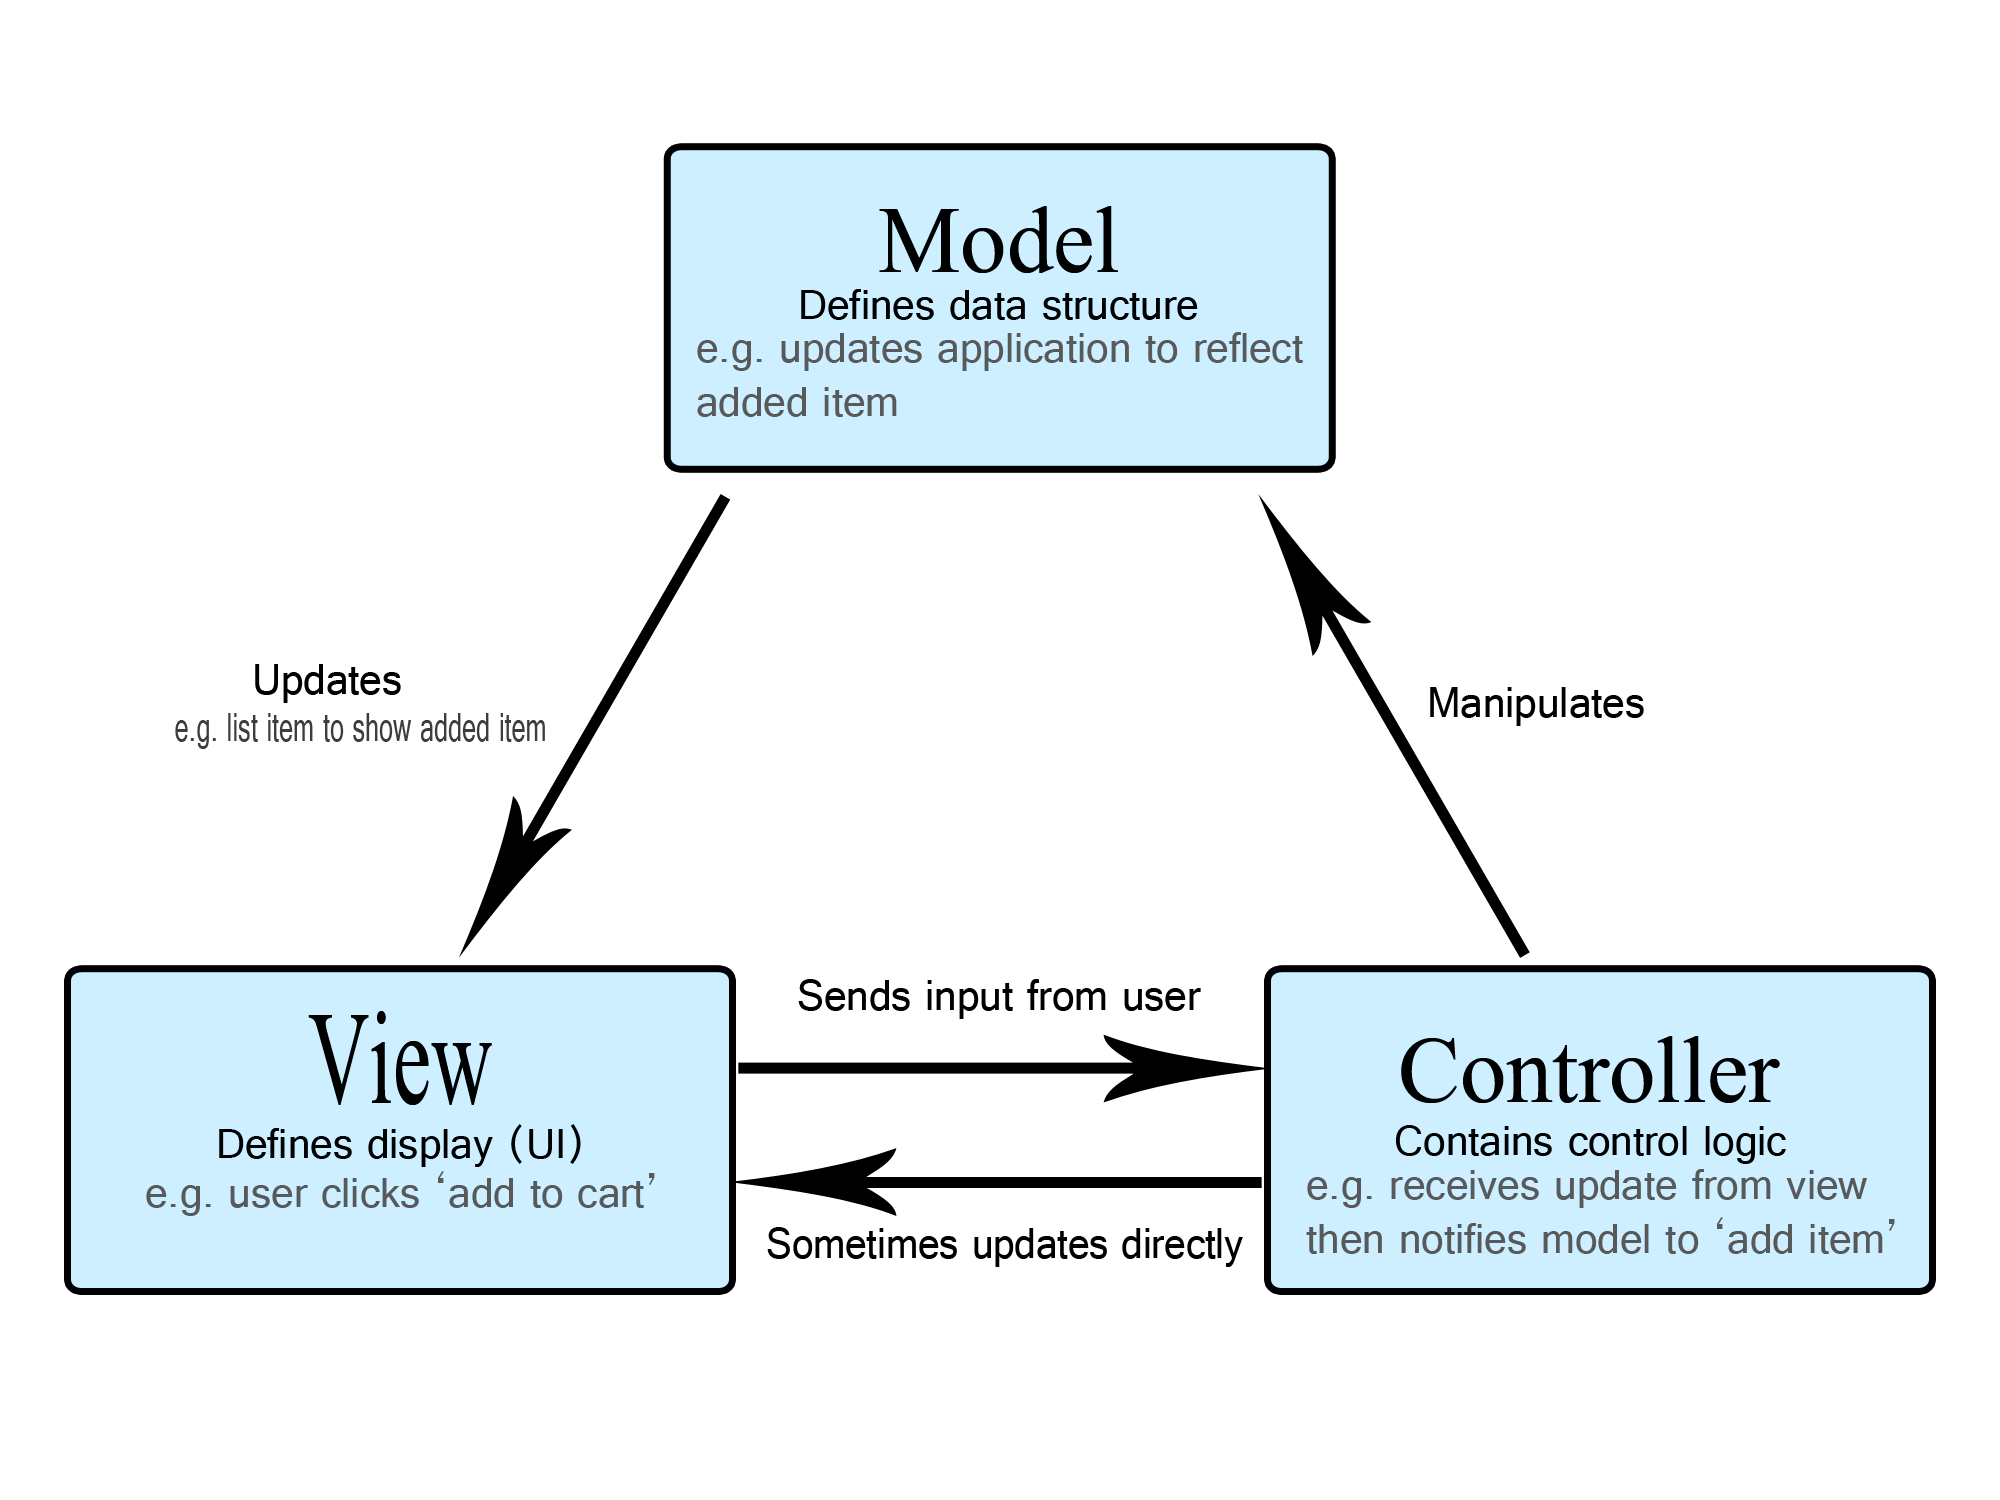
\includegraphics[width=0.70\textwidth]{pictures/mvc.png}
\captionof{figure}{Pattern MVC}
\end{center}
		
\newpage

\subsection{Data Access Object Pattern}
Per la gestione dei dati si è ritenuto di utilizzare il pattern DAO, utilizzato per separare i dati di basso livello che accedono all'API dalle operazioni di alto livello.\\
Per ogni classe del Model (e di conseguenza per quasi tutte le tabelle implementate nel DataBase) si è implementato:
\begin{itemize}
    \item \textbf{Interfaccia DAO} - Definisce le operazioni standard da eseguire.
    \item \textbf{Classe concreta DAO} - Implementa l'interfaccia di cuisopra. È responsabile dell'accesso ai dati dal database.
    \item \textbf{Model Object} - Questo è un semplice oggetto Java che contiene i metodi getter e setter per memorizzare i dati.
\end{itemize}
Le classi-modello implementate con il pattern DAO sono (in ordine alfabetico):
\begin{itemize}
    \item \textbf{ControlPhase} - Fase di Controllo effettuata dal farmacologo.
    \item \textbf{Notice} - gli avvisi ricevuti dal farmacologo.
    \item \textbf{Patient} - i pazienti.
    \item \textbf{Reaction} - le reazioni avverse.
    \item \textbf{RiskFactor} - i fattori di rischio relativi ai pazienti.
    \item \textbf{User} - gli user che hanno accesso all'applicazione (dottori e farmacologi).
    \item \textbf{Vaccination} - le vaccinazioni effettuate dai pazienti.
\end{itemize}

\newpage
\section{Implementazione del DataBase}
Come richiesto dalla traccia si è implementato un database con cui l'applicazione potesse interagire.\\
Il Database è stato creato sulla base dell'ER qui riportato:
\begin{center}
    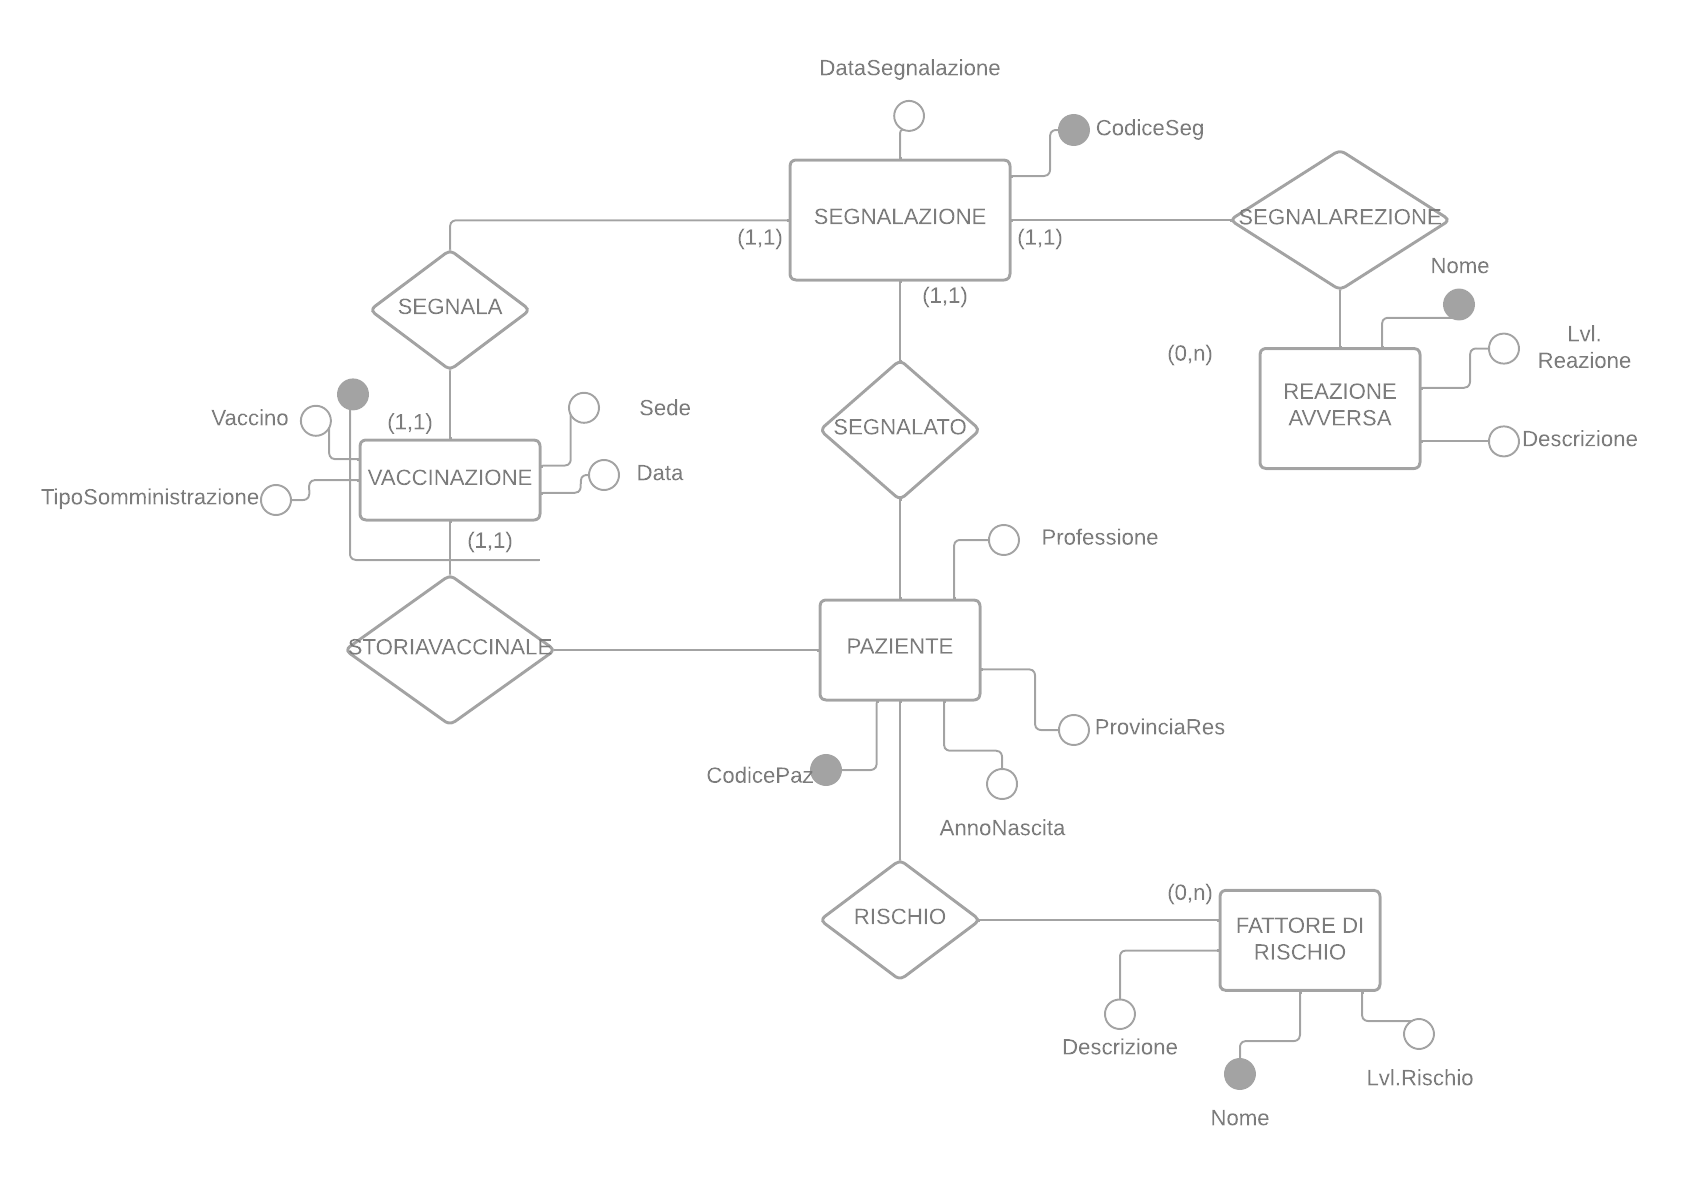
\includegraphics[width=1\textwidth]{pictures/_Diagramma vuoto.png}
    \captionof{figure}{Schema ER da modificare!}
\end{center}
%Aggiungere Relazionale

\newpage
\section*{Appendice A: Query di creazione Database}
\addcontentsline{toc}{section}{Appendice A}

Si è scelto di implementare il Database in PostgreSQL. Riportiamo anche le query usate per la creazione delle tabelle, che ci aiutano a comprendere com'è fatto:
\paragraph*{Tabelle dello schema VaccineSupervisionDB}
\begin{verbatim}
    CREATE TABLE patient(
        idPatient SERIAL PRIMARY KEY,
        birthYear NUMERIC(4) NOT NULL ,
        CHECK ( birthYear >= 1900 ),
        province VARCHAR(20) NOT NULL,
        profession VARCHAR(20) NOT NULL
   );
   
   CREATE TABLE RiskFactor(
       name VARCHAR(20) PRIMARY KEY,
       description VARCHAR(50),
       riskLevel NUMERIC(1) NOT NULL,
       CHECK ( riskLevel >= 1 AND riskLevel <= 5 )
   );
   
   CREATE TABLE Vaccination(
       idPatient INTEGER REFERENCES patient(idPatient),
       vaccine VARCHAR(15) NOT NULL,
       typeSomministration VARCHAR(10) NOT NULL,
       PRIMARY KEY (idPatient, vaccine, typeSomministration),
       vaccinationSite VARCHAR(10) NOT NULL,
       vaccinationDate DATE NOT NULL
   );
   
   CREATE TABLE Reaction(
       name VARCHAR(20) PRIMARY KEY,
       gravity NUMERIC(1) NOT NULL,
       CHECK(gravity >= 1 AND gravity <= 5),
       description VARCHAR(50) NOT NULL
   );
   
   CREATE TABLE PatientRisk(
       idPatient INTEGER NOT NULL REFERENCES patient(idPatient),
       risk VARCHAR(20) NOT NULL REFERENCES RiskFactor(name),
       PRIMARY KEY(idPatient, risk)
   );
   
   CREATE TABLE users(
       username VARCHAR(10) PRIMARY KEY,
       password VARCHAR(12) NOT NULL,
       type BOOLEAN NOT NULL,
       UNIQUE (username, password)
   );
   
   CREATE TABLE Report(
       id SERIAL PRIMARY KEY,
       reportDate DATE NOT NULL DEFAULT CURRENT_DATE,
       reactionDate DATE NOT NULL,
       reaction VARCHAR(20) NOT NULL REFERENCES Reaction(name),
       idPatient INTEGER NOT NULL REFERENCES patient(idPatient),
       doctor VARCHAR(10) REFERENCES users(username)
   );
   
   CREATE TABLE ControlPhase(
       pharmacologist VARCHAR(10) REFERENCES users(username),
       vaccine VARCHAR(15) NOT NULL,
       PRIMARY KEY (pharmacologist, vaccine)
   );
\end{verbatim}

\end{document}